\chapter{Funktionstest}
Nach der Implementierung des zuvor geschilderten Konzepts wurde ein Funktionstest durchgeführt.
Dazu werden zunächst die theoretischen Grenzen der Konfiguration getestet und danach die tatsächlichen Ausgabewerte mit den theoretischen verglichen.
Besonders interessant ist hierbei, in welchem Frequenzbereich der Generator zuverlässig funktioniert.

\section{theoretische Limitierungen}
Um den praktischen Nutzen des Funktionsgenerators einzuschätzen, werden die Grenzen der einstellbaren Frequenz, die Auflösung und der Spannungsbereich berechnet.
Für die Spannung ergeben sich diese Werte aus dem Datenblatt des eingesetzten DACs.
Dieser kann in einem Bereich von 0 bis 5,5 V eingesetzt werden, wobei die Referenzspannung 2,7 V nicht unterschreiten darf \cite{PmodDA2}.
Für den Betrieb auf dem Basys 3-Board läuft der Spannungsbereich von 0 bis 3,3 V, da hier die Ausgangsspannung des Boards der limitierende Faktor ist.
Nachfolgend werden noch der Frequenzbereich und die Auflösung bestimmt.

\subsection{Frequenzbereich}
Der Systemtakt $f_{sys}$ des Generators beträgt 100 MHz.
Der Frequenzbereich der Funktionen, die er ausgeben kann, reicht von ca. 0,0877 Hz bis zu ca. 735 kHz für die Rampen- und Rechteckfunktion.
Für die Zick-Zack-Funktion beträgt $f_{max}$ nur die Hälfte, also ca. 365 kHz.\\

\begin{align}
  f_{count} &= \frac{f_{sys}}{68} \label{test:theo:freq:fcount}\\  
  f_{max} &= \frac{f_{count}}{2}  \label{test:theo:freq:fmax}\\ 
  f_{min} &= \frac{f_{count}}{2^{clk\_width} - 1} \label{test:theo:freq:fmin}
\end{align}

Die Frequenz $f_{count}$ ist die Frequenz mit der der interne Zähler der Funktionsbausteine hochzählt.
Er beträgt ein 64tel des Systemtakts $f_{sys}$ (siehe \cref{test:theo:freq:fcount}).
Die minimale Frequenz $f_{min}$ errechnet sich aus dem maximalen Zählstand, der wiederum abhängig ist von seiner Bitbreite \code{clk\_width} (siehe \cref{test:theo:freq:fmin}).
Die maximale Frequenz ergibt sich aus dem Shannon'schen Abtasttheorem, nach dem die minimale Abtastfrequenz eines Signals doppelt so groß sein muss, wie die Frequenz des abgetasteten Signals.
In diesem Fall entspricht die Abtastfrequenz $f_{count}$ und das abgetastete Signal dem Ausgangssignal, woraus folgt, dass das ausgehende Signal nur halb so groß sein kann, wie $f_{count}$ (siehe \cref{test:theo:freq:fmin}).


\subsection{Auflösung}
Die Auflösung des analogen Ausgangssignals hängt sowohl von der Geschwindigkeit ab, mit der das digitale Signal analogisiert werden kann, als auch von der maximalen Anzahl digital darstellbarer Werte.
Überschreitet die Frequenz des analogen Signals $f$ die Grenzfrequenz $f_{grenz}$, so fällt die Auflösung $R$ reziprok zu $f$ ab (siehe \cref{test:theo:res:plot}).
Oberhalb von $f_{grenz}$ ist die Auflösung durch die Bitbreite des ADCs begrenzt.
Da es sich um einen 12-Bit Wandler handelt, beträgt die Anzahl darstellbarer Werte und damit auch die höchste Auflösung $2^{12} - 1 = 4095$.
Diesen Wert nimmt die Auflösung an, wenn die Frequenz kleiner als $f_{grenz}$ ist (siehe \cref{test:theo:freq:fgrenz}).

\begin{align}
  R &= \begin{cases}
    4095               & f \leq f_{grenz}                      \\
    \frac{f_{count}}{f} & f > f_{grenz} = \frac{f_{count}}{4095} = 359 Hz
        \end{cases} \label{test:theo:freq:fgrenz}
\end{align}

Konkret bedeutet dass für den Funktionsgenerator, dass bei einer Amplitude von $U_{SS}=3,3V$ und einer Frequenz von $f=100kHz$, die Auflösung $4,54V^{-1}$ statt der maximalen Auflösung von $1241V^{-1}$ beträgt, das heißt, dass bei 100kHz 4,54 Werte statt 1241 Werte pro Volt gesampelt werden.

\begin{figure}[h] \centering
    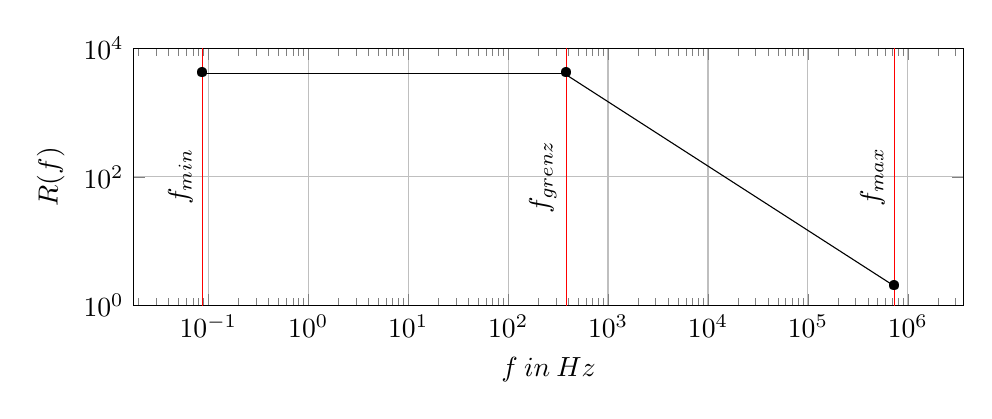
\begin{tikzpicture}
      \begin{loglogaxis}
        [xlabel=$f\:in\:Hz$,
        ylabel=$R(f)$,
        ymin=1,
        ymax=10000,,
        width=\textwidth,
        height=0.4\textwidth,
        grid=major]
        \addplot[color=black, domain=0.08765:359.12] {4095};
        \addplot[color=black, domain=359.12:735294] {100000000 / (68*\x)};
        % help lines and nodes:
        \addplot[color=red] coordinates{(381.12, 1)(381.12, 10000)};
        \node[above, rotate=90] at (381.12, 100) {$f_{grenz}$};
        \node at (381.12, 4095) {\textbullet};

        \addplot[color=red] coordinates{(0.08765, 1)(0.08765, 10000)};
        \node[above, rotate=90] at (0.08765, 100) {$f_{min}$};
        \node at (0.08765, 4095) {\textbullet};

        \addplot[color=red] coordinates{(735294, 1)(735294, 10000)};
        \node[above, rotate=90] at (735294, 100) {$f_{max}$};
        \node at (735294, 2) {\textbullet};
      \end{loglogaxis}
    \end{tikzpicture}
 \caption{Doppelt logarithmisches Diagramm der Auflösung $R(f)$ über den Frequenzbereich $f$. Die Auflösung bleibt konstant bei 4095 1/tick bis sie schließlich bei $f_{grenz}$ anfängt zu sinken.} \label{test:theo:res:plot}
\end{figure}

\section{reales Verhalten}
Nun soll das reale Verhalten des Funktionsgenerators untersucht werden.
Die dazu durchgeführten Versuche sind nachfolgend geschildert.

\subsection{Versuchsaufbau}
Ein Foto des Versuchsaufbaus findet sich in \cref{test:real:setup:pic}.
Das digitale Oszilloskop Analog Discovery 2 von digilent wird an einen Laptop angeschlossen, auf dem dann die Funktionsverläufe mit der Software digilent WaveForms angezeigt werden.

\begin{figure}[h] \centering
  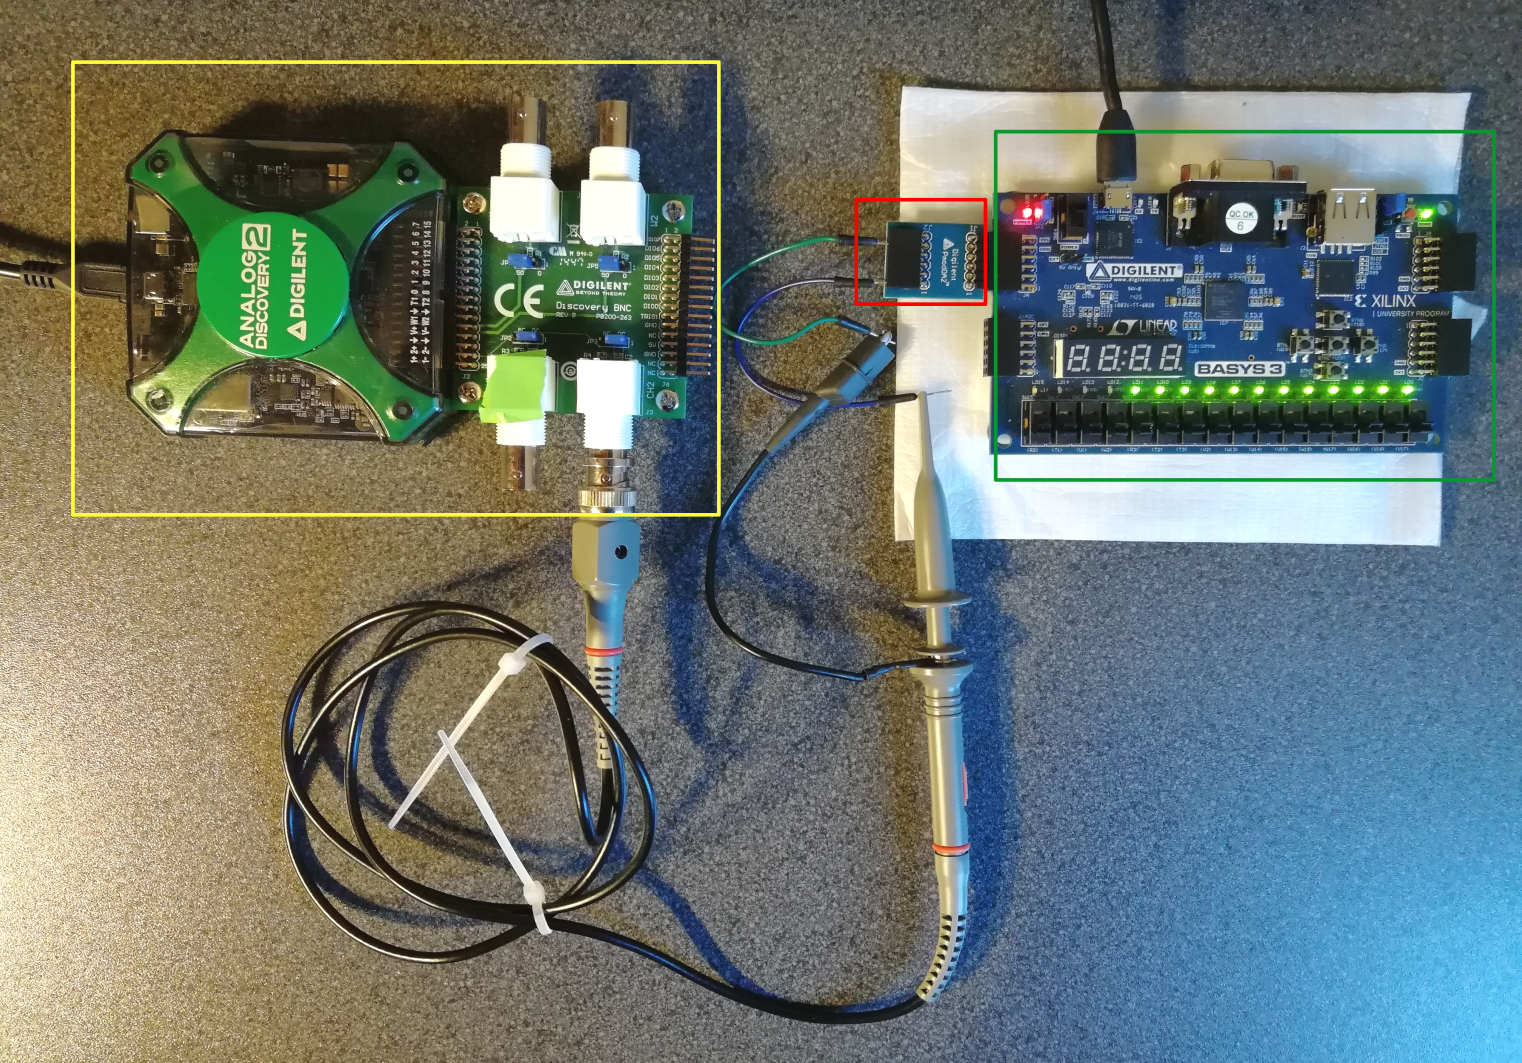
\includegraphics[width=0.8\textwidth]{testaufbau_annotated_fg}
  \caption{Versuchsaufbau zum Testen des Funktionsgenerators. Das Oszilloskop ist mittels des Discovery BNC Moduls (beide gelb umrandet) an den analog Ausgang des PmodDA2-Wandlers (rot umrandet) angeschlossen. Das Basys 3-Board (grün umrandet) wird über das angeschlossene USB Kabel mit Strom versorgt und per UART konfiguriert. Die vom Oszilloskop eingelesenen Daten werden an einen per USB angeschlossenen Laptop (nicht im Bild) verschickt. Die LEDs auf dem Board zeigen den internen digitalen Funktionswert an.}
  \label{test:real:setup:pic}
\end{figure}

\subsection{Versuchsdurchführung}
Um zunächst die korrekte Ausgabe der Funktionsverläufe zu überprüfen, werden alle vier Verläufe nacheinander bei konstanter Frequenz $f=100Hz$ über die UART-Schnittstelle konfiguriert und die erfassten Signale dokumentiert.
Der eingestellte \analog{low} und \analog{high} Wert beträgt 0 bzw. 3,3 V.\\
Anschließend werden alle Funktionen der UART-Schnittstelle überprüft, indem der jeweilige Befehl mit einem dazu passenden Argument abgeschickt wird. \\
Schließlich wird noch der Frequenzbereich anhand der Zick-Zack-Funktion untersucht.
Dazu wird ein Wert knapp unterhalb von $f_{min}$, ($f = 0,08Hz$), und ein Wert oberhalb von $f_{max}$, ($f = 1MHz$), eingestellt.
Dazwischen wird, von 0.1 Hz aufwärts, mit jedem Schritt die eingestellte Frequenz mit 10 multipliziert.
Die Werte für \analog{low} und \analog{high} werden wieder auf 0 und 3,3 V gesetzt.
Auffäligkeiten im Funktionsverlauf werden festgehalten und die Daten werden dann noch im CSV Format für weitere Auswertungen abgespeichert. \\
Um die Frequenz der Zick-Zack Funktion zu messen, werden alle Datenpunkte mitAusgangsspannung $U < 0,5 V$ betrachtet.
Aus den Zeitkomponenten nahe beieinander liegender Punkte wird dann der Mittelwert gebildet.
Die Differenz zweier aufeinanderfolgender Mittelwerte kann als Näherung für die Zykluszeit $T$ betrachtet werden, aus der dann die Frequenz des Signals mit $f = 1 / T$ berechnet wird.

\subsection{Ergebnis}

Zunächst werden Funktionsverläufe bei 100 Hz präsentiert (siehe \cref{test:real:res:plot}).

\begin{figure}[h] \centering
  {
    \pgfplotsset{
    no markers,
    grid=major,
    ymin=-0.2, ymax=3.5,
    scaled x ticks=false,
    ytick={0, 0.55, 1.1, 1.65, 2.2, 2.75, 3.3},
    xtick={-0.005, -0.0025, 0, 0.0025, 0.005},
    xticklabels={-5, -2.5, 0, 2.5, 5},
    width=0.45\textwidth}
  % constant
  \subfloat[][konstante Funktion]{ 
    \begin{tikzpicture}
      \begin{axis}[ylabel=$U(t)$ in V]
        \addplot table [x=Time (s), y=Channel 2 (V), col sep=comma, row sep=newline] {test/const100Hz_small.csv};
      \end{axis}
    \end{tikzpicture}
    \label{test:real:res:plot:const}
  } 
  % square
  \subfloat[][Rechteckfunktion]{
    \begin{tikzpicture}
      \begin{axis}
        \addplot table [x=Time (s), y=Channel 2 (V), col sep=comma, row sep=newline] {test/square100Hz_small.csv};
      \end{axis}
    \end{tikzpicture}
    \label{test:real:res:plot:square}
  } 

  % zigzag 
  \subfloat[][Zick-Zack-Funktion]{
    \begin{tikzpicture}
      \begin{axis}[ylabel=$U(t)$ in V, xlabel=$t$ in ms]
        \addplot table [x=Time (s), y=Channel 2 (V), col sep=comma, row sep=newline] {test/zigzag100Hz_small.csv};
      \end{axis}
    \end{tikzpicture}
    \label{test:real:res:plot:zigzag}
  }
  % ramp
  \subfloat[][Rampenfunktion]{
    \begin{tikzpicture}
      \begin{axis}[xlabel=$t$ in ms]
        \addplot table [x=Time (s), y=Channel 2 (V), col sep=comma, row sep=newline] {test/ramp100Hz_small.csv};
      \end{axis}
    \end{tikzpicture}
    \label{test:real:res:plot:ramp}
  }
}
\caption{Die Ergebnisse des Versuchs bei $f=100Hz$. Die konstante Funktion und die Rechteckfunktion weisen ein leichtes Rauschen auf. Ihr \analog{low} und \analog{high} Wert liegen dauerhaft unter 0 bzw. 3,3 V.} \label{test:real:res:plot}
\end{figure}

Die Verläufe bei $f = 100Hz$ ergaben sich auf den ersten Blick wie erwartet.
Ihre Frequenz wurde mit dem Cursor-Tool der Oszilloskop Software gemessen und ergab ca. 100 Hz.
Jedoch fiel auf, dass \analog{low} und \analog{high} nicht genau 0 bzw. 3,3 V betrugen.
Der Mittelwert des konstanten Signals betrug $\overline{U}_{c}=3,24 V$, beim Rechtecksignal lag der tiefste Wert bei $U_{sl} = -0,11 V$ und der höchste bei $U_{sh} = 3,25 V$, beim Zick-Zack-Signal waren es $U_{zzl} = -0,06 V$ und $U_{zzh} = 3,26 V$ und beim Rampensignal $U_{rl} = -0,1 V$ und $U_{rh} = 3,24 V$. \\
Der Generator ließ sich problemlos per UART konfigurieren.
Alle eingegebenen Befehle führten zu der erwarteten Ausgabe am analogen Ausgang.\\
Beim Abtasten der Frequenz  ergab sich bei Unterschreiten von $f_{min}$ ($f = 0,08Hz$) eine wesentlich höhere Frequenz von 20,5 Hz. 
Im niedrigen Frequenzbereich konnten nur geringe Abweichungen von der eingestellten Frequenz gemessen werden. \\
Je näher $f$ jedoch $f_{max}$ kam, desto stärker wich die gemessene Frequenz $f_{ist}$ von der eingestellten Frequenz $f_{soll}$ ab.
Die Messergebnisse der Frequenzmessung finden sich in \cref{test:real:res:ftab}.

\begin{table}[h]
  \begin{tabular}[h]{|l|r|r|r|r|r|r|r|r|r|r|}
    \hline
    $f_{soll}$ & 0,08 & 0,1 & 1 & 10 & 100 & $10^3$ & $10^4$ & $10^5$ & $3,5 \cdot 10^5$ & $10^6$\\ \hline
    $f_{ist}$ & 20,5 & 0,100 & 1,01& 10,1 & 101 & 999 & $10^4$ & $9,81 \cdot 10^4$ & $2,94 \cdot 10^5$ & - \\ \hline
  \end{tabular}
  \caption{Diese Tabelle stellt die eingestellten Frequenzen $f_{soll}$ in Hz den gemessenen Frequenzen $f_{ist}$ in Hz gegenüber. Für $f_{soll} = 10^6 Hz$ konnte die Frequenz nicht bestimmt werden.} \label{test:real:res:ftab}
\end{table}

Die Verläufe ab einer Frequenz $f > 10 kHz$ wiesen starke Schwankungen auf, die zu einem unsauberen Signal führten (siehe \cref{test:real:res:zzplot}).
Je näher die Frequenz $f_{max}$ kam, desto deutlicher wurde die begrenzte Auflösung, wie in \cref{test:real:res:zzplot:350kHz} zu sehen ist.
Außerdem ändert sich der Wert nicht sprunghaft, sondern eher entsprechend der Ladekurve eines Kondensators.

\begin{figure}[h] \centering
  {
    \pgfplotsset{
    no markers,
    grid=major,
    ymin=-0.2, ymax=3.5,
    scaled x ticks=false,
    ytick={0, 0.55, 1.1, 1.65, 2.2, 2.75, 3.3},
    yticklabels={},
    width=0.37\textwidth}
  \subfloat[][10 kHz]{ 
    \begin{tikzpicture}
      \begin{axis}[ylabel=$U(t)$ in V, xlabel=$t$ in µs,
                   xtick={-0.000075, -0.00005, -0.000025, 0, 0.000025, 0.00005, 0.000075},
                   xticklabels={, -50, , 0, , 50,},
                   yticklabels={0, , 1.1, , 2.2, , 3.3}]
        \addplot table [x=Time (s), y=Channel 2 (V), col sep=comma, row sep=newline] {test/zigzag10000Hz_small.csv};
      \end{axis}
    \end{tikzpicture}
    \label{test:real:res:zzplot:10kHz}
  } 
  \subfloat[][100 kHz]{
    \begin{tikzpicture}
      \begin{axis}[xlabel=$t$ in µs,
        xtick={-0.0000075, -0.000005, -0.0000025, 0, 0.0000025, 0.000005, 0.0000075, 0.000010},
                   xticklabels={, -5, , 0, , 5, , 10}]
        \addplot table [x=Time (s), y=Channel 2 (V), col sep=comma, row sep=newline] {test/zigzag100000Hz_1cyc.csv};
      \end{axis}
    \end{tikzpicture}
    \label{test:real:res:zzplot:100kHz}
  } 
  \subfloat[][350 kHz]{
    \begin{tikzpicture}
      \begin{axis}[xlabel=$t$ in µs,
                   xtick={-0.000004, -0.000002, 0, 0.000002, 0.000004},
                   xticklabels={-4, -2, 0, 2, 4}]
        \addplot table [x=Time (s), y=Channel 2 (V), col sep=comma, row sep=newline] {test/zigzag350000Hz_1cyc.csv};
      \end{axis}
    \end{tikzpicture}
    \label{test:real:res:zzplot:350kHz}
  }
}
  \caption{Signalverläufe ab 10 kHz. Während in \cref{test:real:res:zzplot:10kHz} das Signal noch gut zu erkennen ist, ist es in \cref{test:real:res:zzplot:100kHz} schon sehr undeutlich. In \cref{test:real:res:zzplot:350kHz} liegt die Frequenz schließlich so nah bei $f_{max}$, dass die Auflösung von 4 Schritten erkennbar wird.} \label{test:real:res:zzplot}
\end{figure}

\subsection{Auswertung}
Der Funktionsgenerator gibt die per UART konfigurierten Signale korrekt aus. 
Allerdings scheinen, auch durch den DAC-Konverter, die Genauigkeit und die Bandbreite beschränkt zu sein. \\
Die ungenaue Ausgabe der Spannungswerte \analog{high} und \analog{low} könnte daher kommen, dass der Chip die Versorgungsspannung des Basys 3 Boards als Referenzspannung nutzt.
Da aber mehrere Verbraucher und der Chip selsbt von dieser Spannung gespeist werden, kann sie schnell ungenau werden.
Ein anderer Chip mit einem weiteren Pin für eine Referenzspannung könnte die Genauigkeit erhöhen.
Für einfache Signalverläufe ist sie aber ausreichend. \\
Stellt man die Frequenz auf $f < f_{min}$ ein, so stellt man fest, dass eine größere Frequenz als $f_{min}$ ausgegeben wird.
Dies ist damit zu erklären, dass der interne Zähler eine beschränkte Breite von 24 Bit hat.
Damit beträgt sein maximaler Wert $2^{24} - 1 = 16.777.215$.
Vom Konfigurationswert werden nur die letzten 24 Stellen übernommen, sodass sich der interne Wert wiederum kleiner als $2^{24} - 1$ ist.
Daraus resultiert eine höhere Frequenz als der Nutzer konfigurieren wollte.\\
Die Frequenz zeigt sich bis $f = 10^4 Hz$ stabil, jedoch wird sie zu $f_{max}$ hin sehr ungenau.
Dies ist auf die begrenzte Geschwindigkeit des Zählers der Funktionsbausteine zurückzuführen.
Es können nur Zykluszeiten eingestellt werden, die Vielfache der Zählerzykluszeit sind.
Dieser Umstand fällt dann stärker ins Gewicht, wenn es nur wenige Zyklen abzuzählen gibt, was bei sehr hohen Frequenzen der Fall ist. \\
Auch der ungenaue Signalverlauf lässt sich teilweise mit der begrenzten Zähler-geschwindigkeit und der daraus resultierende sinkenden Auflösung erklären.
Jedoch hätte der Verlauf immer mehr die Form einer Treppe annehmen müssen, da die Auflösung mit steigender Frequenz abnimmt und die Änderung der Spannung pro Konvertierung größer wird.
Eine Ursache für dieses Verhalten kann nicht eindeutig bestimmt werden.
Es könnte daher kommen, dass der DAC-Konverter nicht ausreichend Zeit zur Konvertierung hat.
Andere Fehlerquellen könnten der Messaufbau oder ein Fehler beim versenden der Digitalwerte vom FPGA an den Konverter sein.
Weitere Untersuchungen, eventuell mit einem hochwertigeren Oszilloskop, könnten hier für Erkenntnis sorgen.
